\subsection{\label{sec:stellarium}Stellarium}

In order to check the validity of our livestream-derived optical lightcurve, we needed a way of finding the expected eclipse obscuration percentage over time for our location.
We used the free, open-source planetarium software \texttt{Stellarium}\cite{zotti_simulated_2020} to achieve this.
After setting the time, date and location of our radio telescope in \texttt{Stellarium}, we queried the software's API to step the simulation time forward and extracted the eclipse percentage for 1000 points in time, starting before first contact and ending after fourth contact.
The resulting theoretical lightcurve was then overlaid on the eclipse obscuration derived from the UCA Observatory livestream.
The agreement between the two is excellent, as shown in Figure \ref{fig:OpticalLightcurveComparison}, validating our optical eclipse lightcurve.

\subsection{\label{sec:theoreticalLightcurves}Theoretical Lightcurve Comparison}

To determine the apparent radius of the sun at \unit[1420]{MHz}, we can compare our observed radio lightcurve to a series of theoretical lightcurves where the radius of the sun has been changed.
To accomplish this, we first downloaded high-accuracy ephemeris data from the JPL Horizons On-Line Ephemeris System \cite{nasa_jpl_solar_system_dynamics_group_jpl_nodate}. 
Using the angular radii of both the sun and moon along with the angular separation between the two, we calculated the obscured area of the solar disk at 2000 points in time during the eclipse using the geometric relationships shown in Figure \ref{fig:eclipse_geometry}.
These relationships are also given by Equations 1 through 4.

\begin{figure}
  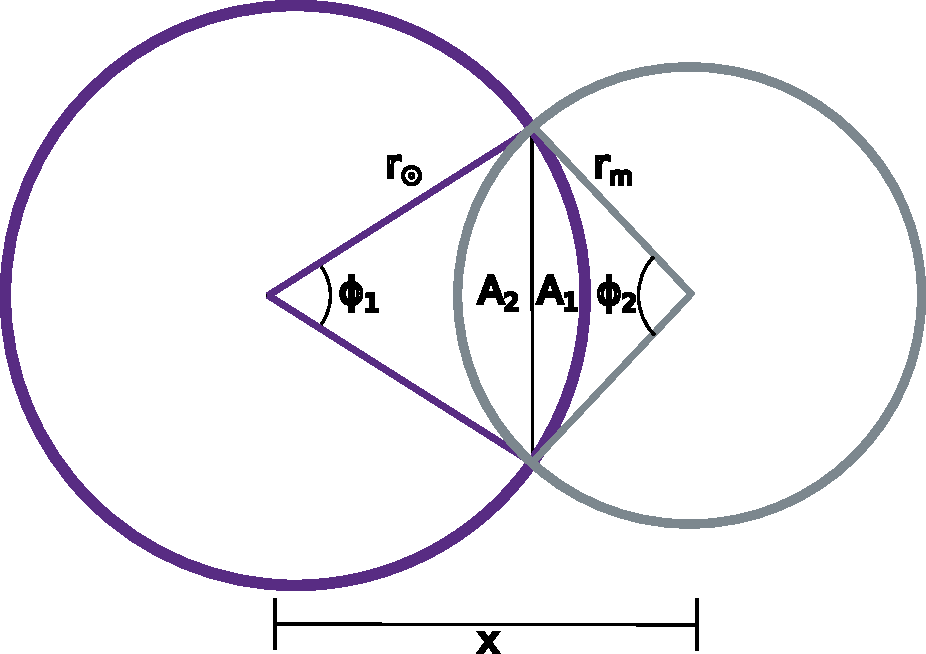
\includegraphics[width=0.5\textwidth]{figures/drawing}
  \caption{\label{fig:eclipse_geometry} The geometric relationships used to calculate the obscuration of the sun.}
\end{figure}

\begin{equation}
  A_1 = \frac{1}{2}r_{\odot}^2\left(\phi_1 - \sin\phi_1\right)
\end{equation}
\begin{equation}
  A_2 = \frac{1}{2}r_{m}^2\left(\phi_2 - \sin\phi_2\right)
\end{equation}

\begin{equation}
  \phi_1 = 2\cos^{-1}\left(\frac{r_{\odot}^2 - r_{m}^2+x^2}{2r_{\odot}x}\right)
\end{equation}
\begin{equation}
  \phi_2 = 2\cos^{-1}\left(\frac{x^2 - r_{\odot}^2 + r_{m}^2}{2r_{m}x}\right)
\end{equation}


\begin{figure}
  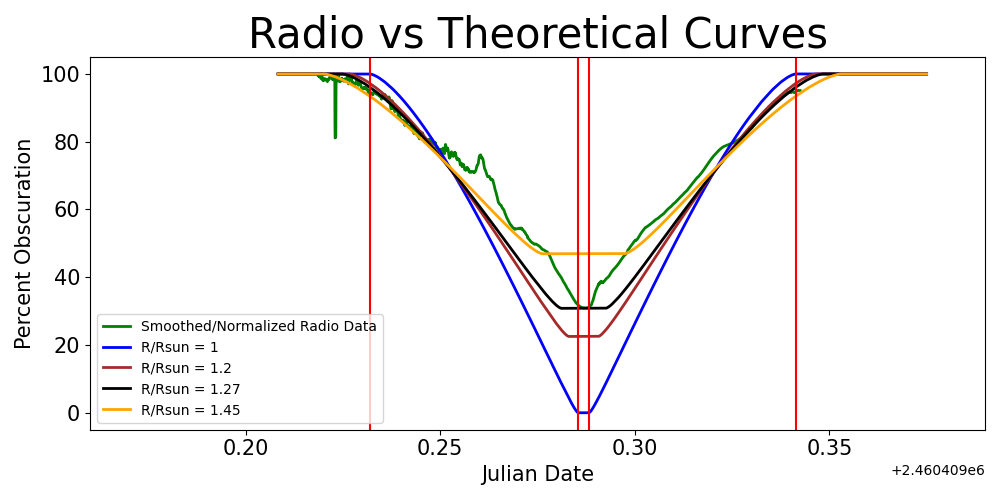
\includegraphics[width=\textwidth]{figures/RadiovsTheoretical.pdf}
  \caption{\label{fig:RadiovsTheoretical} A comparison of the smoothed/normalized radio lightcurve and theoretical lightcurves generated with the JPL Horizons ephemeris data.}
\end{figure}

Our data found that the radio lightcurve reached a minimum of 30.9\% of the total solar flux during totality, whereas the optical lightcurve reached 0\%.
Using these relationships, we were able to create theoretical lightcurves for varying solar radii from $R = 1.0 R_{\odot}$ to $R = 1.45 R_{\odot}$ by calculating the obscured area of the solar disk at 2000 points in time during the eclipse.
These theoretical lightcurves, shown in Figure \ref{fig:RadiovsTheoretical}, helped us match the dip in relative brightness within the radio lightcurve, but it was not a perfect match.
Although the dip in brightness was accurate, the curves show variance in slope.
The theoretical curves assume a uniform disk brightness, not accounting for limb darkening, sunspots, radio emission from the corona, or other solar activity.
Despite these variances, we found that the best-fit curve has an apparent solar radius of $R_{\mathrm{1420}} = 1.27 R_{\odot}$.
This lies between the results of $R_{\mathrm{1420}} = 1.14 R_{\odot}$ found by \cite{messerotti_radio_2000}, and $R_{\mathrm{1420}} = 1.4 R_{\odot}$ found by \cite{leung_solar_2022}.
